\documentclass[../main.tex]{subfiles}

\begin{document}

\chapter{Introduction}
\label{chapter1}
\subsection{Regulation of gene expression}\label{chapter1:regulation-of-gene-expression}
The expression of genes is regulated at several points including transcription, mRNA stability and processing, gene silencing and translation. Transcription is the first level of control and, for many protein\hyp{}coding genes, the rate of transcription will strongly influence
the abundance of the encoded protein~\autocite{liuDependencyCellularProtein2016}. Transcription is controlled by the interactions of certain proteins with DNA regulatory sequences resulting in increases or decreases in gene expression. In eukaryotes, there are two types of DNA regulatory sequences called \textit{cis}\hyp{}regulatory and \textit{trans}\hyp{}regulatory sequences.


\subsubsection{\texorpdfstring{\textit{Cis}-regulatory DNA sequences}{Cis\hyp{}regulatory DNA sequences}}\label{chapter1:cis-regulatory-dna-sequences}
\textit{Cis}\hyp{}regulatory sequences are those on the same molecule of DNA as the gene they regulate. The literature varies when defining \textit{cis}\hyp{}regulatory sequences. For example, \textcite*{wittkoppCisregulatoryElementsMolecular2012} broadly define both promoters and enhancers as \textit{cis}\hyp{}regulatory elements (CREs). This report, in line with \textcite*{swinnenLessonsDomesticationTargeting2016}, defines CREs as small individual motifs within regulatory sequences which can bind to the DNA binding domain of one or more \textit{trans}\hyp{}acting molecules such as transcription factors and non\hyp{}coding RNAs (ncRNAs). Therefore, both transcription factor binding sites (TFBS) and ncRNA binding sites (such as triplex targeting sites) are types of CREs.
A \textit{cis}\hyp{}regulatory module (CRM) is defined as a genomic region encompassing multiple CREs that together regulate an aspect of gene expression pattern~\autocite{guoNewAlgorithmIdentifying2017}. CRMs may include promoters, enhancers, silencers, insulators and locus control regions~\autocite{jeziorskaSystemsBiologyApproach2009}. CRMs can be located within exons~\autocite{tumpelRegulatoryModuleEmbedded2008}, introns~\autocite{ostrovskyIdentificationStrongIntron2018}, 5’\hyp{}untranslated regions (5’UTRs)~\autocite{bolleSegmentsEncodingUntranslated1994,henrySharedCisregulatoryModule2018}, or 3’UTRs~\autocite{palmerEnhancerControlsSnail2007,yochumGenomewideScreenBetacatenin2008} (\autoref{fig:crm}). CRMs can be found tens of kilobases from the core promoter~\autocite{bien-willnerSOX9cre1CisactingRegulatory2007,okaGenomewideMappingTranscriptional2017}, and are still classed as \textit{cis}\hyp{}acting because they are found on the same DNA molecule as the gene they are regulating. In this report, the term CRM will be used to refer to the sequence of DNA upstream of the start codon encompassing both the promoter region and any 5’UTR.

\begin{figure}[!ht]
  \begin{center}
    \capstart
    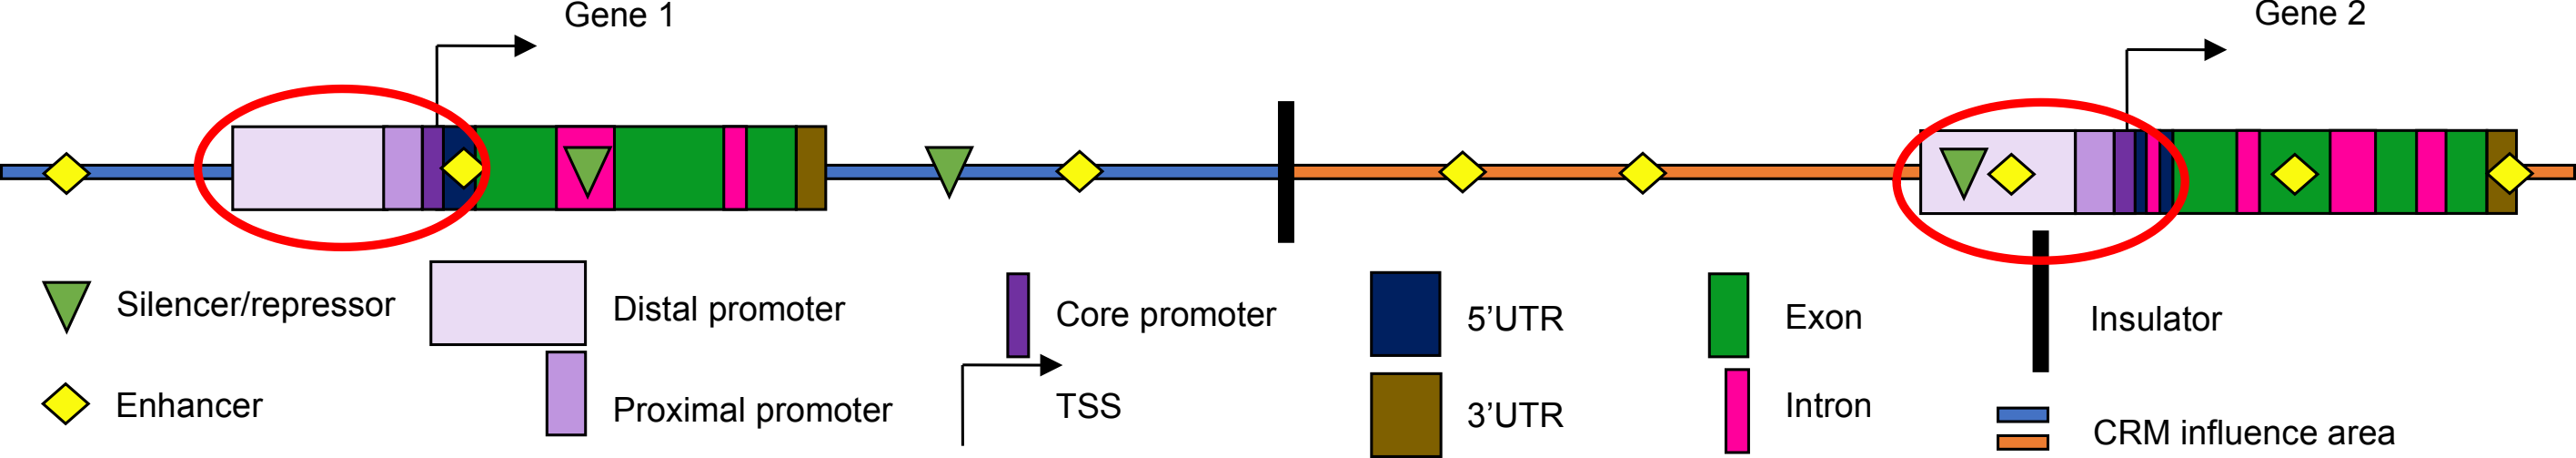
\includegraphics[width=0.70\columnwidth]{crm/crm}
    \caption{\textit{Cis}\hyp{}regulatory module (CRM) classification. CRMs are genomic DNA
      regions containing multiple \textit{cis}\hyp{}regulatory elements such as
      transcription factor binding sites, which together regulate gene
      transcription. UTR, untranslated region. CRMs include promoters,
      silencers and insulators, and can be found within exons, introns, 3'UTRs
      and 5'UTRs. CRM regulation is combinatorial, and can be unique to a
      specific gene or shared between many. Insulators prevent CRMs from
      regulating past that region. Transcription start sites (TSSs) are found
      within the core promoter.
      \label{fig:crm}
    }
  \end{center}
\end{figure}


\paragraph{The promoter}\label{chapter1:the-promoter}
Promoters are essential in establishing baseline transcriptional capacity through the recruitment of proteins such as transcription factors (TFs), which control the recruitment of RNA polymerase II \autocite{portoPlantPromotersApproach2014}.
Promoters can be divided into two classes depending on when and where they are expressed.
Promoters active throughout the majority of developmental stages and environments are classed as constitutive promoters, and those only active in particular tissues (tissue\hyp{}specific) or in response to specific stimuli (inducible) can be termed variable promoters \autocite{bilasCisregulatoryElementsUsed2016}.
TFs bind CREs in a promoter to regulate the spatio\hyp{}temporal pattern of transcription of the downstream gene.
The promoter region can be split into three parts: core, proximal and distal.
The minimal DNA sequence required for transcription initiation is called the core promoter and this is usually spans from -60 to +40 bp relative to the transcription start site (TSS) \autocite{solovyevIdentificationPromoterRegions2010,royCorePromotersTranscription2015}.
\textit{Cis}\hyp{}regulatory elements (CREs) such as the initiator (Inr), TATA box and B recognition Element (BRE) are located in the core promoter.
Motif discovery\hyp{}based analyses hypothesised that general sequence enrichments in the core promoter of plants such as GA elements, CA elements and pyrimidine (Y)\hyp{}patch elements might have a similar function to mammalian promoter CpG (CG) islands \autocite{yamamotoCharacteristicsCorePromoter2011,yamamotoHeterogeneityArabidopsisCore2009}.
CpG sites in CpG islands are unmethylated when genes are expressed, and methylation in CpG sites can silence genes \autocite{birdDNAMethylationPatterns2002}.
In animals, TATA boxes are enriched in variable promoters~\autocite{engstromGenomicRegulatoryBlocks2007,carninciGenomewideAnalysisMammalian2006}, while CpG islands are enriched in constitutive promoters.
Additionally, mammalian constitutive promoters have a higher GC content than responsive promoters~\autocite{vinogradovDNAHelixImportance2017, weiCharacterizationGenePromoters2019}.
The proximal promoter region typically extends ~200\hyp{}300 bp upstream of the TSS and includes the part of the core promoter upstream of the TSS. The proximal promoter region also includes CREs for proteins including transcription factors.
The distal promoter can extend several 1000 bp upstream of the proximal promoter, and contains more CREs. However, these often have weaker influence on transcription than those in the proximal \autocite{pandiarajanVivoPromoterEngineering2018}.

\textcite*{mortonPairedEndAnalysisTranscription2014} used paired\hyp{}end analysis of TSSs (PEAT) to create a
dataset of TSSs from \textit{Arabidopsis thaliana} root samples. This
dataset was used to create a machine learning model called the Plant
PEAT Peaks (3PEAT) model, which predicts the TSS probability at any
given nucleotide. The majority of core plant promoters were found to be
TATA\hyp{}less, and instead contained many other CREs. \textcite*{thieffryCharacterizationArabidopsisThaliana2020} conducted cap\hyp{}analysis gene expression (CAGE) in Arabidopsis which agreed with \SI{95}{\percent} of the PEAT TSSs and was also more sensitive at
detecting more lowly expressed TSSs. Many core promoters contain a
cluster of multiple TSSs called the transcription start region (TSR)~\autocite{carninciGenomewideAnalysisMammalian2006,rachMotifCompositionConservation2009,niPairedendSequencingStrategy2010}. TSRs can be split into classes based on how wide a
region they cover in the core promoter. Narrow regions are associated
with strong, spatio\hyp{}temporal expression, and broader regions with the
weaker expression often associated with constitutively expressed
maintenance genes~\autocite{mortonPairedEndAnalysisTranscription2014}.

\paragraph{The enhancer}\label{chapter1:the-enhancer}

Enhancers increase promoter activity, improving the spatio\hyp{}temporal
specificity of transcription in their target genes. Like promoters,
enhancers are DNA sequences that can contain many CREs recruiting a
variety of TFs and ncRNAs. Enhancers help activate transcription
regardless of their location, orientation or distance from promoters of
genes~\autocite{banerjiExpressionBetaglobinGene1981} (\autoref{fig:crm}). There
are several models explaining how enhancers work: (i) The proteins bound
to enhancers and promoters interact with each other by looping out the
DNA in between them~\autocite{carterLongrangeChromatinRegulatory2002,tolhuisLoopingInteractionHypersensitive2002,vilarDNALoopingGene2005,delaatChapterThreeDimensional2008,amanoChromosomalDynamicsShh2009}.
These interactions form the
transcription initiation protein complexes. This model is the most
highly accepted model. (ii) Enhancers can act by nucleosome remodelling,
supercoiling of DNA, and altering chromatin structure, facilitating the
entry of regulatory proteins to activate transcription~\autocite{corlessEffectsDNASupercoiling2016}. (iii) It has been suggested that both enhancers and
promoters share a common regulatory code, with transcription being
initiated at both~\autocite{coreNascentRNASequencing2008,engreitzLocalRegulationGene2016}. RNA polymerase II binds the core
promoter where it transcribes DNA in both the sense and antisense
directions. This is called bidirectional transcription. At promoters
this typically yields long, stable polyadenylated transcripts in the
sense direction, and short, unstable non\hyp{}polyadenylated transcripts in
the antisense direction~\autocite{anderssonPromoterEnhancerWhat2015}. At enhancers, unstable RNAs
called enhancer RNAs are produced in both directions~\autocite{dingEnhancerRNAsERNAs2018}.
These ncRNAs, along with cohesin, can stabilise long range
enhancer\hyp{}promoter interactions~\autocite{oromLongNoncodingRNAs2010}. In addition, introns
containing enhancers can sometimes be more important than the promoter
for initiating transcription~\autocite{gallegosIntronDNASequences2017}. In \textit{Drosophila}, two
classes of enhancers were identified that were specific to either
constitutively expressed promoters and variable promoters respectively~\autocite{zabidiEnhancerCorepromoterSpecificity2015}.
More than one enhancer can loop to the same promoter, and promoters with more enhancer loop interactions were more conserved than promoters forming fewer enhancer interactions~\autocite{dankoDynamicEvolutionRegulatory2018a}.

\paragraph{The 5'-untranslated region}\label{chapter1:the-5-untranslated-region}

In protein coding genes, the 5'UTR is the stretch of DNA found between a
TSS and the translation start codon. This region is transcribed into
mRNA but is not translated into protein. Plant 5'UTRs can contain a
pyrimidine\hyp{}rich region (5'UTR Py\hyp{}rich stretch) which greatly improves
the transcription rate~\autocite{choudhuryComparativeStudyCultivar2009,duIsolationFunctionalCharacterization2010,bianCloningExpressionCharacterization2011}.
The 5' ends of the mRNAs are
processed by the replacement of the free triphosphate group with a
guanosine triphosphate. Once in place, this 5' cap plays a role in the
recognition of the mRNA by the ribosome~\autocite{byszewskaRNAMethyltransferasesInvolved2014,ramanathanMRNACappingBiological2016}. The mRNAs of
mitochondria~\autocite{temperleyHumanMitochondrialMRNAs2010} and chloroplasts~\autocite{mondeProcessingDegradationChloroplast2000} are
not capped. Once transcribed, the 5'UTR sequence can contain an upstream
open reading frame (uORF) (\SI{50}{\percent} of human 5'UTRs do)~\autocite{calvoUpstreamOpenReading2009},
a guanine\hyp{}rich region~\autocite{beaudoinUTRGquadruplexStructures2010} and an internal ribosome entry
site (IRES)~\autocite{jimenez-gonzalezFunctionalStructuralAnalysis2014}.
Alternative 5'UTRs can be produced via alternative splicing or through
transcription initiation from a different TSS~\autocite{smithPosttranscriptionalRegulationGene2008}.
Because current TSS annotations in the Arabidopsis genome~\autocite{lameschArabidopsisInformationResource2012} are not accurate~\autocite{mortonPairedEndAnalysisTranscription2014,thieffryCharacterizationArabidopsisThaliana2020} and the 5'UTR may contain CREs, it is important to include the 5'UTR in regulatory sequence studies to encompass the whole TSR.

\subsubsection{\textit{Trans}-acting DNA regulation}\label{chapter1:trans-acting-dna-regulation}

A \textit{trans}\hyp{}regulatory sequence is a DNA sequence that contains a
gene encoding for a protein or ncRNA that is used in the regulation of
another target gene~\autocite{watsonRecombinantDNAGenes2007}. \textit{Trans}\hyp{}acting regulation
can involve the specific binding of a \textit{trans}\hyp{}acting molecule such
as a TF or ncRNA to a DNA CRE. Another form of \textit{trans}\hyp{}acting
regulation involves non\hyp{}specific DNA binding by molecules such as
eukaryotic histone proteins in nucleosomes~\autocite{zhangIntrinsicHistoneDNAInteractions2009}.

\paragraph{Sequence specific \textit{trans}-regulation}\label{chapter1:sequence-specific-trans-regulation}

TFs are \textit{trans}\hyp{}acting proteins with domains which bind to TFBSs in
DNA. ncRNAs can contain DNA binding domains which form triple helices
with certain \textit{cis}\hyp{}regulatory elements called triplex target sites
(TTS)~\autocite{kuoDetectionRNADNA2019}. TFs and ncRNAs can contain domains which
interact with other proteins to form complexes which can enhance or
repress gene transcription. Some TFs are able to bind DNA as both
homodimers and heterodimers, increasing regulatory combinations. DNA
regulatory modules such as enhancers can be found on different
chromosomes to the gene they are regulating, where they function in
\textit{trans}~\autocite{geyerTissuespecificTranscriptionalEnhancers1990,xuTransientHomologousChromosome2006,lomvardasInterchromosomalInteractionsOlfactory2006}.

TFs are often part of large families, and many TFs within the same
family can bind to highly overlapping sets of binding sites. TFs from
different families such as bZIPs and bHLHs can compete to bind the same
TFBS~\autocite{toledo-ortizHY5PIFRegulatoryModule2014}. Change in the expression of one TF can
result in cross talk, where the expression of gene targets of other TFs
from the same family are also altered~\autocite{nuruzzamanRolesNACTranscription2013}. Plant TF
families have higher expansion rates than other eukaryotes, not only due
to genome duplications, but also due to increased retention of duplications
within TF families compared to other plant genes~\autocite{shiuTranscriptionFactorFamilies2005}.

An important aspect of TF\hyp{}DNA interactions is the DNA shape. Most
DNA\hyp{}protein interactions occur in the major groove, where bases are most
accessible~\autocite{paboProteinDNARecognition1984}, although some occur in the minor groove~\autocite{bewleyMinorGroovebindingArchitectural1998}. TFs undergo rapid rebinding to ensure the correct orientation is achieved during docking to DNA~\autocite{ganjiDNABindingProteins2016}. The
DNA base cytosine can be methylated, becoming 5\hyp{}methylcytosine (5mC). By
comparing TF binding affinity to TFBSs with and without 5mC, it has been
suggested that TFs might belong to three main groups: (i)
methylation\hyp{}inhibited, (ii) methylation\hyp{}insensitive and (iii)
methylation\hyp{}preferred \autocite{huangPiecingTogetherCisregulatory2018}. Out of \SI{30}{\percent} of
Arabidopsis TFs studied, \SI{76}{\percent} were sensitive to methylation in
their corresponding TFBSs~\autocite{omalleyCistromeEpicistromeFeatures2016}. In a GRN it is important
to incorporate the sequence specific interactions between
\textit{trans}\hyp{}acting molecules, and also between themselves and
regulatory regions in DNA to better understand how to manipulate
networks.

\paragraph{Chromatin}\label{chapter1:chromatin}

Eukaryotic genomes are packed into chromatin, a complex of protein, RNA
and DNA~\autocite{mondalCharacterizationRNAContent2010}, made up of repeating units called
nucleosomes consisting of a histone octamer wrapped around by \num{146} or \num{147}
bp of DNA~\autocite{richmondStructureDNANucleosome2003}. Many DNA CRMs such as promoters and
enhancers are depleted of nucleosomes and some are nucleosome
free~\autocite{struhlDeterminantsNucleosomePositioning2013}. In gene regulatory studies it is important to
incorporate data on non\hyp{}sequence specific interactions between
\textit{trans}\hyp{}acting molecules (\eg{} nucleosome histone proteins) and DNA,
as they reduce how accessible DNA is to other \textit{trans}\hyp{}acting
molecules. Nucleosomes can inhibit the access of TFs to TFBSs. Chromatin
regions highly accessible to DNA\hyp{}binding proteins are called
deoxyribonuclease (DNase) I hypersensitive sites (DHSs) and these can be
mapped following DNase I digestion.

A class of pioneer TFs are able to bind their targets in the presence of nucleosomes.
These pioneer TFs recruit nucleosome remodelers to open up chromatin, allowing previously blocked TFs access to the region~\autocite{zaretPioneerTranscriptionFactors2011}.
In yeast (\textit{Saccharomyces cerevisiae}), stiff DNA poly(dA:dT) regions~\autocite{yuanGenomeScaleIdentificationNucleosome2005,hughesFunctionalEvolutionaryApproach2012} and poly(dG:dC) regions~\autocite{mccallCrystalStructureGGGGCCCC1985} were shown to be depleted of nucleosomes, whereas non\hyp{}homopolymeric GC\hyp{}rich regions favour nucleosome formation~\autocite{struhlDeterminantsNucleosomePositioning2013}.
Yeast promoters containing GC\hyp{}rich motifs and poly(A) motifs concentrated in a narrow region tend to be nucleosome free.
Promoters with the same two motifs in a broader region are characterised by `fragile' nucleosomes, which are less stable.
Fragile nucleosome promoters tend to be highly expressed.
The two motifs have been shown to recruit and/or activate the chromatin structure remodelling complex (RSC) which pushes away flanking nucleosomes, creating a nucleosome free region or space for a fragile nucleosome to form.
To induce nucleosome fragility, Rap1 binding sites were needed upstream of the GC\hyp{}rich and poly(A) motifs~\autocite{kubikNucleosomeStabilityDistinguishes2015}.
Fragile nucleosomes have been detected in maize~\autocite{veraDifferentialNucleaseSensitivity2014} and Arabidopsis~\autocite{passGenomewideChromatinMapping2017}.

\subsubsection{Identification of CREs}\label{chapter1:identification-of-cres}

In order to understand how DNA\hyp{}protein interactions affect gene function it is necessary to understand which proteins bind to specific binding sites in DNA.
Earlier methods involved \textit{in vitro} techniques, however more recent studies identify sites bound by proteins \textit{in vivo}, preserving both context and DNA sequences involved.
A recent \textit{in vitro} method~\autocite{omalleyCistromeEpicistromeFeatures2016} maps protein\hyp{}DNA interactions using DNA retaining \textit{in vivo} features.
Mapping chromatin accessibility and TFBSs helps inform our understanding of gene regulation, and therefore is the basis of understanding and reconstructing gene regulatory networks.

\subsubsection{Identification of chromatin accessible
  regions}\label{chapter1:identification-of-chromatin-accessible-regions}

In the past, it was difficult to annotate non\hyp{}coding DNA regions, and at the genomic scale it was only possible to detect the presence or absence or `regulatory regions'.
As detailed in section \ref{chromatin} (chromatin), CRMs tend to be nucleosome free regions, are very sensitive to digestion by DNase I, and are called DHSs. Many DHS assays have been used to characterise CRMs.
Chromatin accessibility of DNA to DNase I was probed by Southern blotting where, following DNase I digestion, DNA was purified, digested using restriction enzymes, transferred to a membrane then hybridised with radioactively labelled DNA~\autocite{wuChromatinStructureSpecific1979,matherMethylationStatusDNase1983,benderVglobinGeneSwitching2000,wangChromatinStructureMapping2001}.
This was challenging, limited to short stretches of DNA and not very sensitive~\autocite{cockerillIdentificationDNaseIHypersensitive2000}.
DHS methods using PCR (polymerase chain reaction)~\autocite{pfeiferChromatinDifferencesActive1991,fengHighresolutionAnalysisCfos1992} and later quantitative PCR (qPCR)~\autocite{mcarthurQuantificationDNaseIsensitivityRealtime2001,dorschnerHighthroughputLocalizationFunctional2004,martinsTrackingChromatinStates2007} were developed to improve upon the Southern blotting technique for identification of chromatin accessible regions.
DNase I assays were combined with genome\hyp{}wide tiling arrays (DNase-chip) with sequencing~\autocite{crawfordIdentifyingGeneRegulatory2004,saboGenomewideIdentificationDNaseI2004}, and without sequencing~\autocite{crawfordDNasechipHighresolutionMethod2006,saboGenomescaleMappingDNase2006,followsIdentifyingGeneRegulatory2006,shuDistinctModesDNA2012} for genome\hyp{}wide profiling of chromatin accessibility.

As an alternative to DNase assays, a high\hyp{}throughput assay later called formaldehyde\hyp{}assisted isolation of regulatory elements (FAIRE) was developed~\autocite{nagyGenomewideDemarcationRNA2003}.
In this assay, formaldehyde\hyp{}crosslinked chromatin and reference non\hyp{}crosslinked chromatin is extracted using phenol\hyp{}chloroform.
Histone\hyp{}free DNA is collected in the aqueous phase, and enrichment of histone\hyp{}free DNA regions from crosslinked DNA are identified by comparing to the non\hyp{}crosslinked reference on a microarray.

More recent methods combine high\hyp{}throughput sequencing with previous methods, such as DNase-chip with sequencing (DNase I-seq)~\autocite{boyleHighResolutionMappingCharacterization2008} and the FAIRE assay with sequencing (FAIRE-seq)~\autocite{giresiFAIREFormaldehydeAssistedIsolation2007}.
Although DNase-chip was previously combined with sequencing~\autocite{crawfordGenomewideMappingDNase2006}, this only identified \SI{20}{\percent} of DHS sites. Higher throughput sequencing allowed production of genome wide DHS maps~\autocite{boyleHighResolutionMappingCharacterization2008}.
The combination of DNase I-seq with FAIRE-seq to map open chromatin is more effective than either assay alone~\autocite{songOpenChromatinDefined2011}.
DNase I-seq and FAIRE-seq require millions of cells as starting material, with time\hyp{}consuming sample preparations.
This means heterogeneity between cells can be drowned out.
To improve on this, genome\hyp{}wide DNase I-seq has since been scaled down to single cells, called scDNase-seq~\autocite{jinGenomewideDetectionDNase2015}.

The assay for transposase\hyp{}accessible chromatin using sequencing (ATAC\hyp{}seq)~\autocite{buenrostroTranspositionNativeChromatin2013} was developed to require fewer cells in the starting material.
ATAC\hyp{}seq identifies nucleosome\hyp{}bound and nucleosome free regions, along with footprinting of DNA binding proteins.
This method builds on the fact that transposons were shown to integrate into active regulatory regions \textit{in vivo}~\autocite{gangadharanDNATransposonHermes2010}, and uses Tn5 transposase to integrate its adaptor payload into DNA within chromatin accessible regions. ATAC\hyp{}seq uses a simple two\hyp{}step process of Tn5 insertion followed by PCR and sequencing, whereas FAIRE\hyp{}seq and DNase I\hyp{}seq have many more steps and take several days~\autocite{buenrostroTranspositionNativeChromatin2013}.
Single cell ATAC\hyp{}seq (scATAC\hyp{}seq) has also been achieved~\autocite{cusanovichMultiplexSinglecellProfiling2015,buenrostroSinglecellChromatinAccessibility2015}.
The cutting bias of DNase I in DNase I\hyp{}seq~\autocite{heRefinedDNaseseqProtocol2014} and Tn5 transposase in ATAC\hyp{}seq~\autocite{martinsUniversalCorrectionEnzymatic2018} needs to be corrected computationally when analysing data~\autocite{liuLongNoncodingRNA2019a}.

ATAC\hyp{}seq and DNase I\hyp{}seq identify regions of open chromatin which correlate to nucleosome occupancy.
Nucleosome occupancy itself can be profiled genome\hyp{}wide using micrococcal nuclease digestion followed by sequencing (MNase\hyp{}seq) \autocite{weberH2ANucleosomesEnriched2010,henikoffEpigenomeCharacterizationSingle2011,pajoroProfilingNucleosomeOccupancy2018}.
In Mnase\hyp{}seq, DNA is digested using MNase unless it is protected by nucleosomes.
Protected DNA can then be sequenced in a high\hyp{}throughput manner to identify nucleosome sites.
An alternative to MNase\hyp{}seq called NOMe\hyp{}seq (nucleosome occupancy and methylome sequencing)~\autocite{kellyGenomewideMappingNucleosome2012} uses GpC methyltransferase which methylates GpC dinucleotides not protected by nucleosomes or strongly binding proteins.
Native methylation uses CpG dinucleotide cytosine methylation, whereas the added GpC methyltransferase methylates GpC dinucleotide cytosines.
Using this information, both nucleosome occupancy and endogenous DNA methylation can be obtained simultaneously.

\subsection{Identification of specific DNA-protein
  interactions}\label{chapter1:identification-of-specific-dna-protein-interactions}

DNase I is used to footprint DNA\hyp{}protein interactions.
\textit{In vitro} DNase I footprinting is where radioactively labelled DNA fragments are incubated with and without the protein of interest, then digested with DNase I and analysed by electrophoresis and autoradiography~\autocite{galasDNAseFootprintingSimple1978}.
Bound proteins protect the DNA backbone from digestion by DNase I, allowing identification of specific binding sites of proteins on DNA.
Another method for characterising DNA\hyp{}protein interactions is the electrophoretic mobility shift assay (EMSA)~\autocite{garnerGelElectrophoresisMethod1981}, which quantifies the binding of proteins to DNA.
A fragment of DNA containing a putative TFBS is fluorescently or radioactively labelled and is run on a polyacrylamide gel with and without the protein of interest.
DNA\hyp{}protein complexes run more slowly on the gel than DNA on its own.

More recent techniques include systematic evolution of ligands by exponential enrichment (SELEX).
SELEX is an \textit{in vitro} assay where libraries of randomly generated nucleic acid ligands of fixed length are flanked by 5' and 3' primers~\autocite{tuerkSystematicEvolutionLigands1990}.
The oligonucleotide library is exposed to a protein of interest, unbound oligos are removed, and then oligos are amplified using PCR.
This cycle is repeated several times until the oligo population is enriched for ones which bind protein.
These are then identified and characterised.
SELEX has recently been modified to investigate the location and orientation of TFBSs in DNA wrapped around nucleosomes, with a technique called nucleosome consecutive affinity purification (NCAP)\hyp{}SELEX~\autocite{zhuInteractionLandscapeTranscription2018}.
This uses SELEX to enrich nucleosome bound DNA, and then DNA is incubated with TFs.
Using nucleosome and TF tags, DNA is separated based on whether or not it is bound by nucleosomes and TFs, and is then sequenced.
This infers whether the addition of a certain TF affects the stability of the nucleosome, and identifies TF binding specificities and positions on nucleosomal DNA.

Chromatin immunoprecipitation (ChIP) was developed to map protein\hyp{}DNA crosslinking \textit{in vivo}.
There are two types of ChIP, differentiated by starting input.
XChIP uses chromatin fixed with formaldehyde and sheared by sonication~\autocite{solomonMappingProteinDNAInteractions1988,orlandoMappingChromosomalProteins2000}, and NChIP uses native chromatin from nuclei digested by micrococcal nuclease~\autocite{hebbesDirectLinkCore1988}.
Protein specific antibodies are then used to pull down the protein of interest bound to DNA.
The resulting DNA sequences are then purified and analysed using Southern blot, PCR or qPCR~\autocite{dasChromatinImmunoprecipitationAssay2004}, although PCR bias may mean AT\hyp{}rich sequences are amplified more than GC\hyp{}rich ones~\autocite{weinmannIdentificationUnknownTarget2002}.
NChIP is most useful for mapping the DNA target of histone modifiers, while XChIP is most useful for mapping TF\hyp{}DNA interactions.
Even so, some TF\hyp{}DNA interactions have been successfully mapped using NChIP~\autocite{gregoryDNAMethylationLinked2001}.
ChIP has been combined with sequencing to identify DNA sequences where proteins bind~\autocite{weinmannUseChromatinImmunoprecipitation2001}, and also combined with DNA footprinting, to identify specific TFBSs~\autocite{leekangCombiningChromatinImmunoprecipitation2002}.
Although these methods accurately identify TFBSs in DNA, a drawback is that they are very low throughput.

To increase throughput, ChIP was combined with whole\hyp{}genome microarrays (ChIP\hyp{}chip), creating high resolution genome wide maps of DNA\hyp{}protein interactions~\autocite{weinmannIsolatingHumanTranscription2002,wellsIdentificationNovelPRb2003,renGenomeWideLocationFunction2000}.
\textcite*{buckChIPchipConsiderationsDesign2004} provide an excellent review of this.
Briefly, XChIP is carried out, and DNA fragments enriched for protein binding are purified and fluorescently labelled.
Genomic DNA prepared by immunoprecipitation is used as a reference, amplified, and labelled with a different tag.
The two probes are hybridised onto a single DNA microarray.
Areas of the genome enriched for DNA\hyp{}protein binding are identified, and exact binding sites can be predicted \textit{in silico}~\autocite{liuAlgorithmFindingProtein2002}.

ChIP\hyp{}chip is limited in that only a subset of TFBSs are retrieved due to the array design.
Also, ChIP\hyp{}chip is restricted to species for which whole\hyp{}genome tiling arrays have been made.
With the advance of high\hyp{}throughput sequencing technology, these limitations were overcome through the development of ChIP\hyp{}seq, where ChIP DNA is sequenced in a high\hyp{}throughput way, providing greater sensitivity, resolution and specificity than ChIP\hyp{}chip~\autocite{johnsonGenomeWideMappingVivo2007}.

ChIP\hyp{}seq provides genome\hyp{}wide TFBS mapping for specific TFs.
Even so, TFBS information is available for relatively few TFs.
This is because ChIP\hyp{}seq is not scalable for high\hyp{}throughput identification of 1000s of TF\hyp{}DNA interactions as it is dependent on antibody quality, is difficult for lowly expressed proteins and is challenging to perform~\autocite{kidderChIPSeqTechnicalConsiderations2011}.

Another method of identifying DNA-protein interactions is DNA adenine methyltransferase identification (DamID)~\autocite{steenselIdentificationVivoDNA2000}. DamID uses the \textit{E. coli} DNA adenine methyltransferase (Dam) fused to a TF or chromatin protein of interest.
Wherever the protein of interest binds, even transiently, Dam methylates adenine in GATC motifs~\autocite{sanchez-romeroDNAMethylationBacteria2015}.
DNA is then extracted and fragmented by the methylation sensitive restriction endonuclease DpnI.
Methylated sequences are then amplified by PCR and then sequenced.
DamID and ChIP methods are fundamentally different.
DamID shows where a protein has previously been in close proximity to DNA, even transiently, while ChIP shows where a protein binds DNA at a given time point.
DamID is good for identifiying DNA-protein interactions which are low in abundance, while ChIP methods struggle to pick them up.
ChIP on the other hand is good for profiling DNA-protein interactions at short time intervals, while Dam-fusions require expression for several hours to achieve sufficient methylation~\autocite{augheyDamItGood2016}.

The protein binding microarray (PBM) is another method of identifying TF-DNA interactions developed by \textcite*{bulykProteinBindingMicroarrays2007}. In this method, a TF of interest is expressed with an epitope tag which is purified and then applied to a DNA microarray. Any non-bound protein is washed away and then the microarray is stained with a primary antibody specific to the epitope tag. The signal intensity can be quantified as it corresponds to the number of DNA-protein binding events. PBM analysis was utilised in Arabidopsis to identify DNA binding motifs for 63 TFs~\autocite{franco-zorrillaDNAbindingSpecificitiesPlant2014}.

The recently developed \textit{in vitro} DNA affinity purification sequencing (DAP-seq) offers a scalable alternative to ChIP and increased specificity compared to motifs generated by PBMs and SELEX~\autocite{omalleyCistromeEpicistromeFeatures2016}.
DAP\hyp{}seq uses \textit{in vitro} expressed TFs to find binding locations on genomic DNA retaining its \textit{in vivo} properties.
Briefly, a genomic DNA library is prepared by attaching a small DNA sequencing adaptor onto purified, fragmented genomic DNA.
Separately, affinity\hyp{}purified TFs are prepared by \textit{in vitro} expression.
The DNA library is added to each specific TF, and unbound DNA is washed away.
The bound fraction is amplified and sequenced.
Reads are mapped to a reference genome and enriched peaks are used to identify TFBSs.
As this uses genomic DNA, which contains cell, tissue and organism specific methylation, methylation preferences of TFs can be mapped.
This is done using a modified DAP\hyp{}seq protocol called ampDAP\hyp{}seq, where a DNA library has any modifications removed by use of a PCR step.
This data can be compared to DAP\hyp{}seq data to assess the methylation preferences of TF binding~\autocite{omalleyCistromeEpicistromeFeatures2016}.

Methods like ChIP, DamID, PBMs and DAP-seq are TF\hyp{}centred methods.
The yeast one\hyp{}hybrid (Y1H) assay is a DNA centred method to identify proteins binding the DNA~\autocite{liIsolationORC6Component1993}.
It involves a report construct where the promoter DNA of interest (termed the bait) is placed upstream of a reporter protein.
A TF of interest (termed the prey) is fused to a yeast transcription activation domain and is expressed in an expression construct.
Both constructs are introduced to a yeast strain, and if the TF of interest binds the DNA of interest then the yeast activator domain induces the reporter expression.
The downside of Y1H assays is that they do not identify whether a TF of interest activates or represses a promoter~\autocite{reece-hoyesYeastOnehybridAssays2012}.
The throughput of Y1H assays were enhanced using a robotic mating platform~\autocite{reece-hoyesEnhancedYeastOnehybrid2011}.
Recently, this enhanced Y1H assay was used in plants to elucidate interactions between nitrogen-responsive genes~\autocite{gaudinierTranscriptionalRegulationNitrogenassociated2018}.

The \textit{in vitro} techniques such as DAP-seq, Y1H and PBMs fail to account for \textit{in vivo} features such as chromatin structure, protein-protein interactions and TF combinations.
The \textit{in vivo} method ChIP does not show whether a TF-DNA interaction leads to gene expression, and it often poorly predicts TF regulation~\autocite{brooksNetworkWalkingCharts2019}.
TF perturbation using overexpressing or knockout transgenic lines are one way of validating targets but these methods are time consuming and do not scale well in eukaryotes.
It is also not possible to distinguish direct from indirect targets.
A technique called transient assay reporting genome\hyp{}wide effects of transcription factors (TARGET) was developed in plant protoplasts~\autocite{bargmannTARGETTransientTransformation2013}.
Briefly, the TF of interest is fused to a glucocorticoid receptor (GR) and expressed transiently in protoplasts.
The expression plasmid also contains a separate expression cassette with red fluorescent protein (RFP) enabling fluoresence\hyp{}activated cell sorting (FACS) of transformed protoplasts~\autocite{bargmannFluorescenceActivatedCell2010}.
The GR-TF fusion is held in the cytoplasm by HSP90-GR binding. Dexamethasone (DEX) is added which disrupts the HSP90-GR binding and induces nuclear localisation of the TF.
Target gene induction after DEX treatment with and without the presence of a translation inhibitor, cycloheximide (CHX), is measured using qPCR analysis.
This shows direct and indirect gene regulation.
Recently, the TARGET method was scaled up using an empty vector control allowing 24 TF assays per day (8 TFs with 3 replicates)~\autocite{brooksNetworkWalkingCharts2019}.
All samples including the empty vector were treated with CHX, mitigating the need to compare CHX positive and negative samples.
Cells separately transfected with either RFP or green fluorescent protein (GFP) were pooled in pairs, allowing the simultaneous FACS of two TFs in each well.
After FACS, RNA-seq analysis was used to identify activated or repressed targets.
However, this scaled up method only detects direct targets.
It is necessary to combine TF-target methods to fully illucidate connections in GRNs.
A time\hyp{}series micro-ChIP protocol for use with small cell samples~\autocite{dahlMChIPRapidMicro2008} was modified for use with the TARGET assay~\autocite{paraMChIPSeqGenomeWideMapping2018} allowing both methods to be run on the same samples~\autocite{paraHitandrunTranscriptionalControl2014, doidyHitandRunTranscriptionNovo2016}.
A recent study combined micro-ChIP, DamID and the TARGET assay allowing transiently bound targets of the NLP7 TF to be identified five minutes after nuclear localisation of the TF~\autocite{alvarezTransientGenomewideInteractions2020}.
These studies also utilised 4-thiouracil (4tU) labelling of nascent transcripts~\autocite{sidaway-leeDirectMeasurementTranscription2014}, allowing affinity-based capture of \textit{de novo} synthesised RNA.
By monitoring TF-DNA interactions over time and using 4tU labelling and steady\hyp{}state RNA-seq these two methods showed that targets of bZIP1 and NLP7 continued to be actively transcribed even after the TFs dissociated from their targets.

In Arabidopsis, recent DNase I\hyp{}seq data~\autocite{sullivanMappingDynamicsRegulatory2014} was published, predicting active regulatory regions where many TFs can bind.
The development of DAP\hyp{}seq has characterised specific TFBSs from a third of Arabidopsis TFs~\autocite{omalleyCistromeEpicistromeFeatures2016}.
Therefore, TFBS data can now be overlayed with the DNase I\hyp{}seq footprint data to map regulatory regions in Arabidopsis.
TFBSs can also be predicted \textit{de novo} with software that can construct position weight matrices (PWMs) describing the binding motifs of a TFs, such as MEME~\autocite{baileyFittingMixtureModel1994}, and the faster STEME~\autocite{reidSTEMEEfficientEM2011}.
Motif prediction has a high false positive rate~\autocite{zambelliMotifDiscoveryTranscription2013}.
Algorithms such as RPMCMC~\autocite{ikebataRepulsiveParallelMCMC2015} and DREME~\autocite{baileyDREMEMotifDiscovery2011} offer cofactor motif discovery, which for example can predict whether TFs form homo and heterodimers when they bind.
In 2015, convolutional neural network (CNN) models were able to learn filters similar to PWM motif matching, and these algorithms outperformed PWM algorithms~\autocite{alipanahiPredictingSequenceSpecificities2015}.
An unpublished CNN model incorporates TF\hyp{}TF interactions during its TFBS prediction~\autocite{lanchantinPrototypeMatchingNetworks2017}.

\subsection{Evolution of gene regulation}
{\label{chapter1:evolution-of-gene-regulation}}

Investigations into the DNA conservation landscape have identified
conserved DNA regions within populations and across species, and this is
because of selection pressure. Evolutionary selection pressure is higher
for coding exon sequences than it is for non\hyp{}coding regulatory sequences
such as the promoter, 5' and 3'UTRs in mammals~\autocite{lindblad-tohHighresolutionMapHuman2011} and
plants~\autocite{haudryAtlas900002013}. However, functional motifs such as TFBSs
within non\hyp{}coding regions exhibit high levels of evolutionary
conservation~\autocite{zhaoConservedMotifsPrediction2012}. When these functional motifs change,
for example due to random mutations called single nucleotide
polymorphisms (SNPs), they can cause changes in expression
level~\autocite{rockmanAbundantRawMaterial2002} and potentially even network
rewiring~\autocite{liEvolutionTranscriptionNetworks2010}. This can be through a change in the
affinity of TFs to the TFBS, addition or deletion of sites, change in
the spacing of TFBSs, or change in nucleosome conformation in the area~\autocite{fyonEnhancerRunawayEvolution2015}.

Some genes may have multiple copies in the genome, which express
products with similar functions~\autocite{guRapidDivergenceExpression2002}. In redundant copies,
the selection pressure on motifs in their non\hyp{}coding regions may be
reduced, resulting in random mutations accumulating in the motifs. These
gene copies therefore may have different spatio\hyp{}temporal expression
patterns~\autocite{forcePreservationDuplicateGenes1999}. These different expression patterns could
have evolved following genome expansion. New genes can be formed through
evolutionary whole genome duplications, creating ohnologues.
Additionally, small\hyp{}scale duplications (SSDs) can occur. One such
example is tandem duplication, which creates consecutive gene copies in
the genome due to unequal crossing over~\autocite{freelingBiasPlantGene2009}. Other SSDs
include retroposed duplicates, created through RNA\hyp{}mediated
retroposition; proximal duplicates, where duplicate genes are separated
by a few genes; and dispersed duplicates, where duplicates are found
throughout the genome, not in syntenic homologous chromosome
regions~\autocite{arsovskiEvolutionCisRegulatoryElements2015}.

There are two types of genetic events affecting gene regulation: (i)
those caused by point mutations of existing sequences, and (ii) those
caused by genome expansion driven by transposable elements, genome
duplications and small scale duplications (SSDs)~\autocite{marnettoEvolutionaryRewiringHuman2018}. Once duplicated, mutations can arise in one paralogue turning it into a
non\hyp{}functional pseudogene~\autocite{zhangEvolutionGeneDuplication2003}. If the original gene had
several functions, these can be shared between both paralogues, in a
process called subfunctionalisation. Regulatory subfunctionalisation can
occur where paralogues retain the same function but tissue specific
expression patterns become shared between them. Another possibility
following gene duplication is that one paralogue can acquire a new
function whilst the other maintains its original function, which is
called neofunctionalisation. In regulatory neofunctionalisation, one
paralogue acquires a novel expression pattern, while the other keeps its
original expression pattern. Duplicated genes can undergo both neo- and
subfunctionalisation~\autocite{heRapidSubfunctionalizationAccompanied2005}. Duplicated genes can also both
maintain ancestral function and expression pattern, adding to robustness
of their regulatory network~\autocite{guRoleDuplicateGenes2003}. However, gene
duplication can cause fragility in GRNs, instead of improving their
robustness. This may be he case if the function of the protein of one
paralogue becomes dependent on the presence of the other~\autocite{dissGeneDuplicationCan2017}. Hypofunctionalisation has also been proposed, where
the expression level of the paralogues decreases, meaning both copies
are required for normal function~\autocite{qianMaintenanceDuplicateGenes2010,veitiaGeneDuplicatesAgents2017}.

Mutations within CREs of duplicated genes are the likely cause of
regulatory neo- and subfunctionalisation~\autocite{arsovskiEvolutionCisRegulatoryElements2015}. Recently,
duplicated genes in yeast were shown to quickly gain TFBSs after
duplication~\autocite{tsaiEvolutionCisregulatoryElements2012}. Additionally, it has been suggested that
in all eukaryotic diploid organisms, enhancer strength may increase in a
runaway fashion due to the competition for expression between homologous
enhancer alleles~\autocite{fyonEnhancerRunawayEvolution2015}. In plants, the distribution of
known core promoter elements with respect to the TSS is conserved within
monocots and dicots~\autocite{kumariGenomeWideComputationalPrediction2013}.

\subsection{Engineering regulation}\label{engineering-regulation}

\subsubsection{Development of synthetic regulatory elements for
  microbes}\label{chapter1:development-of-synthetic-regulatory-elements-for-microbes}

Many studies have described the assembly and characterisation of
promoter libraries for microbes. For example, in \textit{E. coli} ,
directed evolution was used to engineer a broad range of precise
promoter strengths~\autocite{alperTuningGeneticControl2005}. Promoters made in this way tend
to have a broad host range~\autocite{jensenSequenceSpacersConsensus1998}. Combinatorial libraries
of random promoter architectures has also been achieved in \textit{E.
  coli~}~\autocite{coxProgrammingGeneExpression2007}. They show that gene expression can be
regulated by over five orders of magnitude. The location of regulatory
elements within a promoter was key to determining the expression level,
with those located closer to the TSS more effective than those further
away. Some regulatory elements were dominant over others when located in
the same promoter. More directed semi\hyp{}rational promoter engineering
focussed on retaining the consensus sequence of TFBSs, and mutating
spacers~\autocite{jensenSequenceSpacersConsensus1998}. Rational promoter design increased \textit{E.
  coli} promoter activity through the addition of a TFBS~\autocite{zhangDesignDynamicSensorregulator2012}. A synthetic promoter utilising an AND gate, where it
is only activated in the presence of two TFs, was also created
in \textit{E. coli}~\autocite{wangEngineeringModularOrthogonal2011}. A ratiometric expression assay was
used in \textit{E. coli} to characterise gene expression level, by
measuring activity of promoters compared to a reference, and variation
between experiments was reduced by \texttildelow\SI{50}{\percent} \autocite{kellyMeasuringActivityBioBrick2009}.

Synthetic promoter libraries in the yeasts \textit{Komagataella
  pastoris}~\autocite{hartnerPromoterLibraryDesigned2008} and \textit{S. cerevisiae}~\autocite{nevoigtEngineeringPromoterReplacement2006} showed that promoter strength could be changed by introducing mutations in TFBSs. Synthetic promoters were used to study nucleosome occupancy
effects on transcription, and allowed the rational design of synthetic
promoters with increased transcription~\autocite{curranDesignSyntheticYeast2014}. A massively
parallel reporter assay (MPRA) was used to test semi\hyp{}random 312 bp
constitutive and 246 bp responsive promoters in \textit{S. cerevisiae},
where conserved regions containing TFBSs remained the same~\autocite{kotopkaModeldrivenGenerationArtificial2020}. Machine
learning facilitated the \textit{in silico} design of new promoters of
specific expression levels, including expression higher than in any of
the test data set used to train the model. When tested \textit{in
  vivo} these designed promoters had similar expression levels to the
predicted values. Synthetic minimal yeast promoter
libraries were generated to identify minimal upstream activating
elements, and this led to the development of a promoter reduced by \SI{80}{\percent}
in size which still achieved high expression levels~\autocite{reddenDevelopmentCharacterizationSynthetic2015}.

The use of synthetic TFs allows control of gene expression
heterologously in many systems, and allows the design of tissue specific and
or constitutive promoters, as synthetic TFs can themselves be controlled
by tissue specific or constitutive promoters. Synthetic TFs have been
created in yeast using zinc fingers~\autocite{khalilSyntheticBiologyFramework2012}, with a
methodology allowing construction of an unlimited number of different
synthetic TFs. Transcriptional output was tuned through modification of
zinc finger binding sites in promoters, as well as through modifications
to the zinc finger protein itself. Later, inducible synthetic
transcription activator\hyp{}like effectors (TALEs) and dCas9\hyp{}based synthetic
TFs together with small synthetic promoters were trialled, also in yeast~\autocite{machensSyntheticPromotersTranscription2017}. Synthetic TFs have been designed using zinc fingers in \textit{E. coli} too~\autocite{husseyProgrammableT7basedSynthetic2018}. This enabled activation of promoters, rather than de\hyp{}repression of promoters which had been used in
the past, as bacterial promoters are generally on by default~\autocite{browningLocalGlobalRegulation2016}.

\subsubsection{Synthetic regulatory elements for plants}\label{chapter1:synthetic-regulatory-elements-for-plants}

Promoter studies in yeast~\autocite{reddenDevelopmentCharacterizationSynthetic2015,boerDecipheringEukaryoticGeneregulatory2019,kotopkaModeldrivenGenerationArtificial2020} and human cell lines~\autocite{mattioliHighthroughputFunctionalAnalysis2019} often rely on high\hyp{}throughput testing of randomised promoters to identify synthetic promoters with the desired characteristics.
High\hyp{}throughput reporter assays such as massively parallel reporter assays (MPRAs) are not currently achievable in plants, even in plant protoplasts, as it is not guaranteed that a cell will not receive more than one promoter.
Therefore, the rational design of synthetic promoters is required in plants.

Ratiometric expression assays in plants can be achieved~\autocite{brucknerLibrarySyntheticTranscription2015}, in a way similar to that done in \textit{E. coli}~\autocite{kellyMeasuringActivityBioBrick2009}, which increases the resolution of expression characterisation.
This can be used to validate the expression of synthetic promoters.
Synthetic promoters were used to study flanking sequence changes of tissue\hyp{}specific CREs in rice~\autocite{wangNovelGreenTissuespecific2015}.
This identified functional expression pattern changes, and led to the design of five synthetic promoters which were specific to different
green tissues.
Increasing the number of TFBSs in pathogen\hyp{}inducible synthetic promoters increased transcription in Arabidopsis~\autocite{rushtonSyntheticPlantPromoters2002}.
However, too many repeated \textit{cis}\hyp{}regions in a promoter led to an increase in background induction of promoters, possibly by increasing basal level of transcription through allowing increased binding of normally low affinity TFs.
Increased motif copy number was also shown to increase expression in tobacco~\autocite{sawantVarietySynergisticAntagonistic2005} and rice~\autocite{wuGCN4MotifRice1998a}.

As well as microbes~\autocite{khalilSyntheticBiologyFramework2012}, synthetic zinc finger TFs were successfully developed in multicellular eukaryotes such as Arabidopsis~\autocite{guanHeritableEndogenousGene2002}.
More recently, a library of synthetic transcription activator\hyp{}like effector (TALE)\hyp{}activated promoters has been developed in plants~\autocite{brucknerLibrarySyntheticTranscription2015}, demonstrating a range of promoter strengths.
Synthetic dCas9-based TFs have also been used in plants~\autocite{piatekRNAguidedTranscriptionalRegulation2015}.

\subsubsection{Towards engineering regulation in plants}\label{chapter1:towards-engineering-regulation-in-plants}
%read https://www.sciencedirect.com/science/article/pii/B9780444640857000101 to update this section
Promoter engineering can be divided into two approaches to generate novel promoters: i) library generation for random promoter mutagenesis, and ii) generation of \textit{de novo} promoters.
Recent studies have shown that genetic variation can be created in plants via pooled transformation of CRISPR-Cas9 libraries~\autocite{jacobsGenerationCollectionMutant2017,luGenomewideTargetedMutagenesis2017,mengConstructionGenomeWideMutant2017,jacobsGenerationCollectionMutant2017,baiGenerationMultiplexMutagenesis2020}. The development of a near PAM (protospacer\hyp{}adjacent motif)\hyp{}less Cas9 will allow even more variation to be introduced~\autocite{waltonUnconstrainedGenomeTargeting2020}. Tissue\hyp{}specific mutations in certain cell types can also be generated by using CRISPR tissue-specific knockout (CRISPR-TSKO), allowing lethal knockout genes to be studied, and allowing tissue-specific hypotheses to be tested in the future~\autocite{decaesteckerCRISPRTSKOTechniqueEfficient2019}.

Using the various synthetic biology approaches detailed above, catalogues of standardised parts, such as synthetic promoters and TFs, can be produced~\autocite{patronStandardsPlantSynthetic2015}, and then these can easily be used to rewire gene regulatory networks.
Since the recent development of DAP\hyp{}seq and DNase I\hyp{}seq datasets in Arabidopsis, more accurate mapping of TFBSs is achievable, which will help in the design of synthetic regulatory sequences for fine tuning of gene regulation.
Precise genome editing tools such as transcription activator-like effector nucleases (TALEN) and clustered regularly interspaced palindromic repeats (CRISPR)-Cas systems can be used to edit plant genomes~\autocite{malzahnPlantGenomeEditing2017}.
Improved editing can make specific changes to CRMs, allowing easier testing of regulatory hypotheses.
These genome editing techniques can also be deployed as synthetic transcription factors such as TALE- and dCas9\hyp{}based TFs.
Spatio\hyp{}temporal design of promoters will allow specific expression patterns, and the range of expression levels of synthetic promoters will allow for specific regulation in synthetic circuits.
Synthetic regulation of transcription will allow network rewiring by altering native TF\hyp{}DNA networks, and will also allow incorporation of synthetic circuits which do not interfere with endogenous networks.

\subsection{Aims and experimental approach}\label{chapter1:aims-and-experimental-approach}

The main aim of this project is to determine how CREs evolve and to
explore if and how changes in plant gene regulatory sequences can
generate novel expression patterns and rewire gene\hyp{}regulatory networks.
To investigate these questions, three approaches are being taken:

In the first approach, I am comparing CRM architecture (specifically in
promoter and 5'UTR) of constitutively expressed genes to variable genes.
Specifically, I will find changes in the identity, context and frequency
of TFBSs within the CRMs.

\textbf{Hypotheses:}

\begin{itemize}
  \tightlist
  \item
        \textit{Cis}\hyp{}regulatory modules of variable genes will have a lower
        percentage of bp covered by at least one TFBS than CRMs of
        constitutive genes.
  \item
        Constitutive CRMs will have a more diverse TFBS profile than variable
        CRMs both for TF family and individual TFs as they will require a
        wider range of TF binding to be actively expressed across many
        different tissues and conditions
  \item
        Variable genes will be enriched for TATA boxes compared to
        constitutive genes
  \item
        Constitutive promoters will have a higher GC content than variable promoters
  \item
        Constitutive promoters will be more conserved than variable promoters
\end{itemize}

In the second approach, I am designing and testing variants of plant
regulatory sequences to determine how changes in primary sequences
affect the affinity of TFs to their target motifs and how this affects
expression of the target gene. To do this, a CRISPR library will be
constructed and delivered to add variation to the promoter of a nitrogen
response master regulator. Mutations causing changes to expression and
phenotype will be investigated to see if they fall within TFBSs. If they
do, co\hyp{}expression analyses of transient promoters with and without the
mutations along with their cognate TF will be tested using a rapid,
transient ratiometric protocol in Arabidopsis leaf and root
protoplasts that has previously been established in the laboratory. This
will test whether the promoter still responds to the TF after being
mutated. Changes in the affinity of TFs for their target sequences will
be investigated using electrophoresis mobility shift assays (EMSA) and,
in the future, using a novel plate\hyp{}based protein\hyp{}DNA affinity assay
currently being developed by colleagues.

\textbf{Hypotheses:}

\begin{itemize}
  \tightlist
  \item
        Mutations to the core elements of TFBSs will reduce or eliminate TF
        binding.
  \item
        Changes to the position or sequence context of TFBS may increase or
        reduce the affinity of TFs for their target sequences resulting in
        changes (amplitude or tissue specificity) to gene expression.
  \item
        {Disrupted TFBSs closest to the transcription start site (TSS) will
        have the greatest influence on the rate of transcription.}
  \item
        Information about the identity, context and frequency of TFBSs will
        enable the engineering of endogenous regulatory sequences to alter the
        expression levels and tissue\hyp{}specificity of genes, including TFs which
        may result in large\hyp{}scale transcriptional remodelling.
\end{itemize}

In the third approach, genetic feedback will be engineered into the
N\hyp{}response network. A synthetic promoter containing binding sites for a
nitrate\hyp{}responsive TF will be generated. To validate the functionality
of the synthetic promoter, its expression will be tested tested with and
without the co\hyp{}expression of its cognate TF for expression changes using a transient ratiometric protocol in Arabidopsis protoplasts.
The affinity of the TF to the target sequence will also be tested.
dCas9\hyp{}activators and repressors binding to the promoter of a nitrate\hyp{}response master regulator will be introduced as transgenes under the control of the synthetic N\hyp{}responsive promoter, introducing positive or negative feedback.
The gene expression and plant phenotype will be analysed.

\textbf{Hypotheses:}

\begin{itemize}
  \tightlist
  \item
        The synthetic promoter will respond more strongly to nitrogen when it contains more TFBSs for the same N\hyp{}responsive TF.
  \item
        Positive and negative feedback can be engineered into the nitrogen pathway leading to a faster or slower response to nitrate.
  \item
        The engineered feedback will cause expression changes and a change in plant phenotype
\end{itemize}

\end{document}